要使得流水线具有良好的性能,必须使流水线畅通流动,不发生断流。但由于流水过程中会出现以下3种相关冲突,因此实现流水线的不断流是困难的。这3种相关是\textbf{资源相关(结构相关)、数据相关和控制相关。}

{\textbf{1.资源相关(结构相关)}}

所谓资源相关是指多条指令进入流水线后在同一机器时钟周期使用了\textbf{同一个功能部件所发生的冲突}。假定一条指令流水线由5段组成,分别为取指令(FI),指令译码(ID)、计算有效地址或执行(EX)、访存取数(MEM)和结果写寄存器(WB),见下表。

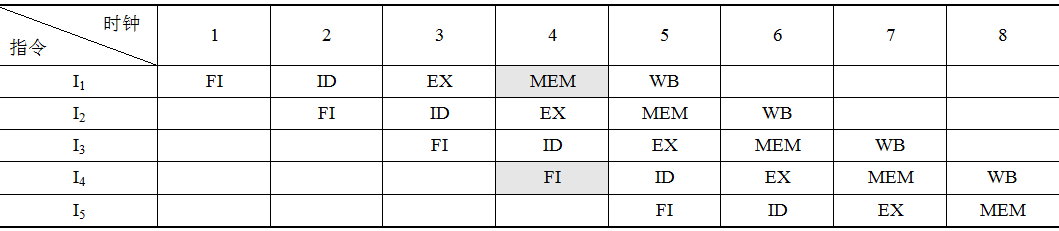
\includegraphics[width=6in]{png-jpeg-pics/C656872B483E2D129A4BF3617641FC50.png}

在第4个时钟,第
\includegraphics[width=0.13542in,height=0.13542in]{texmath/a7b7ddI1}条的MEM段(访存取数)与第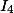
\includegraphics[width=0.14583in,height=0.13542in]{texmath/e32a4cI4}条的FI段(访存取指令)都要访问存储器。当数据和指令放在同一个存储器且只有一个访问口时,便发生两条指令争用存储器资源的相关冲突,\textbf{有两个办法解决冲突:}

{\textbf{方法1:第I4条的FI段停顿一个时钟再启动。}}

{\textbf{方法2:增加一个存储器,将指令和数据分别放在两个存储器中。}}

{\\
}

{{\textbf{2.数据相关(重中之重)}}}

{{\textbf{(1)写后读相关}}}

{字面理解就是应该先写入再读取,而现在是没有写入就已经读了(即{读了旧数据}),出现错误。}

{\textbf{(2)读后写相关}}

{字面理解就是应该先读取再写入,而现在是写入后再读取({本来应读取旧数据,现在却读到了新数据}),出现错误。}

{\textbf{(3)写后写相关}}

{字面上理解是前面一条指令先写数据,然后后面一条指令再写,而现在恰好相反了,导致数据错误。}

{\textbf{3.控制相关}}

\textbf{控制相关冲突是由转移指令引起的。}当执行转移指令时,依据转移条件的产生结果,可能顺序执行下一条指令;也可能转移到新的目标地址取指令,从而使流水线发生断流。

{\textbf{解决方式:}}采用``猜测法''技术,机器先选定转移分支中的一个,按它取指并处理,条件码生成后,如果猜测正确,那么流水线继续进行下去;如果猜测错误,那么之前预取的指令失效。
